% =====================================================================
%  rs_muscl.tex -- the manual's figure of chapter 5 (Method RS): the
%  order-2 reconstruction of one quantity (u or P) over five cells of
%  equal mass, between a ghost on each side. Built by 'make manual'.
%  Cell averages W = 1.0, 1.3, 2.4, 3.0, 2.7 (M = 1). Van Leer slopes
%  s = 2ab/(a + b) when ab > 0, else 0 (module rs, vanleer):
%    cell 1: beside a ghost, s = 0
%    cell 2: a = 0.3, b = 1.1, s = 0.66/1.4 = 0.47143
%    cell 3: a = 1.1, b = 0.6, s = 1.32/1.7 = 0.77647
%    cell 4: a = 0.6, b = -0.3, a peak, s = 0
%    cell 5: beside a ghost, s = 0
% =====================================================================
\documentclass[tikz,border=6pt]{standalone}
\usepackage{amsmath}
\usetikzlibrary{arrows.meta}
\definecolor{slate}{HTML}{2C3E50}
\definecolor{oiblue}{HTML}{0072B2}
\definecolor{oiorange}{HTML}{E69F00}
\begin{document}
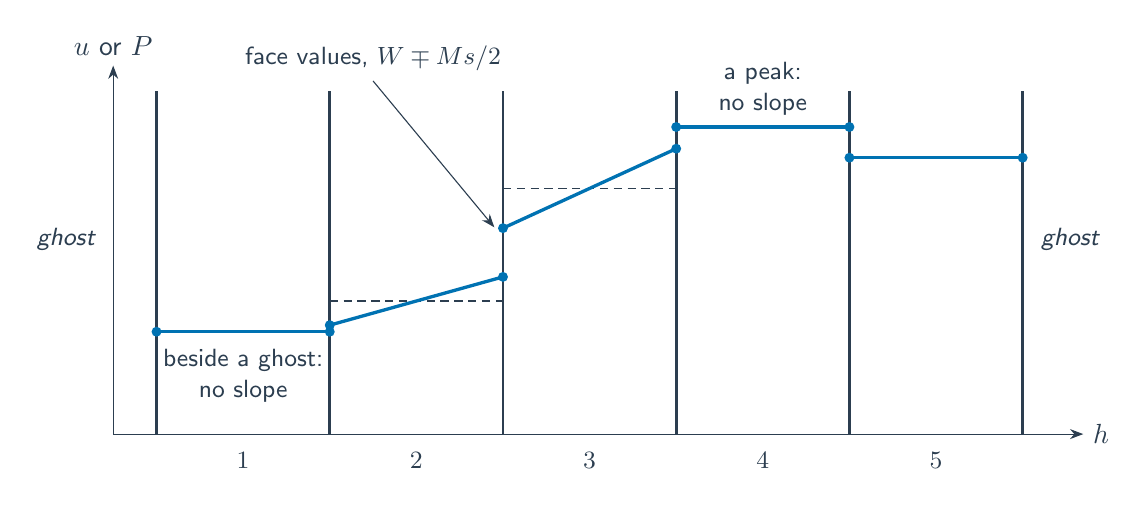
\begin{tikzpicture}[font=\sffamily, text=slate, >=Stealth,
    x=2.2cm, y=1.3cm]
  % axes
  \draw[->, slate, thin] (-0.25,0) -- (5.35,0) node[right] {$h$};
  \draw[->, slate, thin] (-0.25,0) -- (-0.25,3.6) node[above] {$u$ or $P$};
  % faces
  \foreach \f in {0,1,2,3,4,5}
    \draw[slate, line width=1.0pt] (\f,0) -- (\f,3.35);
  % ghost labels
  \node[slate, font=\sffamily\small\itshape, anchor=east] at (-0.3,1.9) {ghost};
  \node[slate, font=\sffamily\small\itshape, anchor=west] at (5.05,1.9) {ghost};
  % cell averages (dashed) and limited lines (solid)
  \foreach \k/\w/\s in {1/1.0/0, 2/1.3/0.47143, 3/2.4/0.77647,
                        4/3.0/0, 5/2.7/0} {
    \draw[slate, densely dashed, thin] ({\k-1},\w) -- (\k,\w);
    \draw[oiblue, very thick] ({\k-1},{\w-0.5*\s}) -- (\k,{\w+0.5*\s});
    \fill[oiblue] ({\k-1},{\w-0.5*\s}) circle (1.8pt);
    \fill[oiblue] (\k,{\w+0.5*\s}) circle (1.8pt);
    \node[below=3pt, font=\sffamily\small] at ({\k-0.5},0) {$\k$};
  }
  % annotations
  \node[font=\sffamily\small, anchor=south, align=center] at (3.5,3.02)
    {a peak:\\ no slope};
  \node[font=\sffamily\small, anchor=north, align=center] at (0.5,0.92)
    {beside a ghost:\\ no slope};
  \node[font=\sffamily\small, anchor=south, align=center] (fv) at (1.25,3.45)
    {face values, $W \mp M s/2$};
  \draw[slate, thin, ->] (fv.south) -- (1.95,2.02);
\end{tikzpicture}
\end{document}
